% ju 28-Mai-22
\documentclass[a4paper,12pt,fleqn,parskip=half]{scrartcl}
\usepackage[ngerman]{babel}
\usepackage[utf8]{inputenc}
\usepackage[T1]{fontenc}

% Schrift
%\usepackage{lmodern}
\usepackage[osf,sc]{mathpazo} 
\usepackage[scale=.9,semibold]{sourcecodepro}   
\usepackage[osf]{sourcesanspro}  

\usepackage[headsepline]{scrlayer-scrpage}
\pagestyle{scrheadings}
\clearpairofpagestyles

\usepackage[table,dvipsnames,usenames]{xcolor}
\usepackage{textcase}
\usepackage{nameref}
\usepackage{hyperref}
\usepackage{tabularx}
\usepackage{multirow}
\usepackage{multicol}
\usepackage{caption, booktabs}
\usepackage{graphicx} 
\usepackage{scrhack}    
\usepackage{url}%% Links
\usepackage[inline]{enumitem}
\usepackage{pifont}
\usepackage{eurosym}% \euro 20,-
\usepackage{amsmath}
\usepackage{amsfonts}
\usepackage{amssymb}
\usepackage{array}            % Extending the array and tabular environments
\usepackage{chngcntr}         % Change the resetting of counters
\usepackage[version=4]{mhchem}
\usepackage{stmaryrd}
\usepackage{siunitx}
\usepackage{float}
\usepackage{csquotes}
\usepackage{subcaption}
\usepackage{mathtools}
\usepackage{icomma}%Dezimaltrennzeichen
\usepackage{multimedia}%Video: \movie[externalviewer]{(video.mov)}{video.mov}
\usepackage{epstopdf}
\usepackage{footnote}
\usepackage{qrcode}% Anwendung: \qrcode[hyperlink,level=Q,version=2,height=1cm]{\website}
\usepackage{underscore}% Unterstrich ____

% PDF Dokumente einbinden
\usepackage{pdfpages}% \includepdf[pages=-]{Tabellen/Excel.pdf}
\RequirePackage{lastpage}  % Pagecounter

\addto\captionsngerman{%
\renewcommand{\figurename}{Abb.}
\renewcommand{\tablename}{Tab.}
}

% listings
\usepackage{listings}
\lstset{basicstyle=\linespread{1}\ttfamily\small,floatplacement=!htb,captionpos=t,abovecaptionskip=.5\baselineskip,belowcaptionskip=.5\baselineskip,upquote=true,showstringspaces=false,inputencoding=utf8,tabsize=4,
    	keywordstyle=\bfseries ,
	commentstyle=\color{rot5},
	stringstyle=\color{orange},
	breaklines=true,
  	postbreak=\mbox{\textcolor{black}{$\hookrightarrow$}\space},
	breakatwhitespace=false
}
\lstset{literate={á}{{\'a}}1 {é}{{\'e}}1 {í}{{\'i}}1 {ó}{{\'o}}1 {ú}{{\'u}}1 {Á}{{\'A}}1 {É}{{\'E}}1 {Í}{{\'I}}1 {Ó}{{\'O}}1 {Ú}{{\'U}}1 {à}{{\`a}}1 {è}{{\`e}}1 {ì}{{\`i}}1 {ò}{{\`o}}1 {ù}{{\`u}}1 {À}{{\`A}}1 {È}{{\'E}}1 {Ì}{{\`I}}1 {Ò}{{\`O}}1 {Ù}{{\`U}}1 {ä}{{\"a}}1 {ë}{{\"e}}1 {ï}{{\"i}}1 {ö}{{\"o}}1 {ü}{{\"u}}1 {Ä}{{\"A}}1 {Ë}{{\"E}}1 {Ï}{{\"I}}1 {Ö}{{\"O}}1 {Ü}{{\"U}}1 {â}{{\^a}}1 {ê}{{\^e}}1 {î}{{\^i}}1 {ô}{{\^o}}1 {û}{{\^u}}1 {Â}{{\^A}}1 {Ê}{{\^E}}1 {Î}{{\^I}}1 {Ô}{{\^O}}1 {Û}{{\^U}}1 {œ}{{\oe}}1 {Œ}{{\OE}}1 {æ}{{\ae}}1 {Æ}{{\AE}}1 {ß}{{\ss}}1 {ű}{{\H{u}}}1 {Ű}{{\H{U}}}1 {ő}{{\H{o}}}1 {Ő}{{\H{O}}}1 {ç}{{\c c}}1 {Ç}{{\c C}}1 {ø}{{\o}}1 {å}{{\r a}}1 {Å}{{\r A}}1 {€}{{\EUR}}1 {£}{{\pounds}}1 {~}{{\textasciitilde}}1 {-}{{-}}1 }

% bibliography
\usepackage[
    bibencoding=utf8,
    backend=biber,% bibtex, biber
    backref=false,backrefstyle=three+,url=true,urldate=comp,abbreviate=false,maxnames=20
]{biblatex} %Paket laden
\DeclareBibliographyCategory{cited}
\let\defaultcite\cite\renewcommand*\cite[2][]{\addtocategory{cited}{#2}\defaultcite[#1]{#2}}
\let\defaulttextcite\textcite\renewcommand*\textcite[2][]{\addtocategory{cited}{#2}\defaulttextcite[#1]{#2}}
\setcounter{biburllcpenalty}{7000}
\setcounter{biburlucpenalty}{8000}
\AfterPackage{biblatex}{
	\PreventPackageFromLoading[\errmessage{Sie haben versucht, das Cite-Paket zu laden, das nicht mit biblatex kompatibel ist.}]{cite}
}

\hypersetup{%
	%pdftitle={\titel},
	%pdfsubject={Latex},
	%pdfauthor={\autor},
	%pdfcreator={\autor}, 
	bookmarksnumbered=true,
	breaklinks=true,
	%colorlinks=true,	   
	linkcolor=rot5,		
	filecolor=blau5,		
	urlcolor=blau5,			
	citecolor=ForestGreen
}

\linespread{1.1}
\setlist{itemsep=0pt}
\widowpenalty10000
\clubpenalty10000
\tolerance1000   

\usepackage[left=2cm,right=2cm,top=1cm,bottom=1cm,includeheadfoot]{geometry}
%\usepackage[left=4cm,right=2cm,top=1cm, bottom=1cm,includeheadfoot]{geometry}
%\usepackage[left=6cm,right=1cm,top=1cm, bottom=1cm,includeheadfoot]{geometry}
%\usepackage[landscape=true,left=2cm,right=2cm,top=1cm,bottom=1cm,includeheadfoot]{geometry}%quer

% eigene Farbe definieren
% Adobe Prozessfarben: CMYK: 100,50,0,35 -> 1,0.5,0,0.35
\definecolor{orange}{cmyk}{0,0.55,0.61,0}   % 0,55,61,0
\definecolor{blau5}{cmyk}{1,0.77,0.1,0.01}  % 100,77,10,
\definecolor{rot5}{cmyk}{0.22,1,1,0.19}     % 22,100,100,19
\definecolor{grau2}{cmyk}{0,0,0,0.1}        % 0,0,0,40
\definecolor{blau}{cmyk}{0.93,0.66,0,0.21}% 

% Literatur
\bibliography{content/literatur}
\bibliography{content/literatur-kfz}
\bibliography{content/literatur-sport}

%%%%%%%%%%%%%%%%%%%%%%%%%%%%%%%%%%%%%%%%%%%%%%%%%%%%%%%
\newcommand{\name}{Jan Unger}% anpassen!!!!!
\newcommand{\thema}{FM_U07_gemischte_Schaltung_Loesung}% anpassen!!!!!
\newcommand{\quelle}{\name}
\newcommand{\website}{https://bw-ju.de/}
\newcommand{\github}{https://github.com/ju1-eu}
%%%%%%%%%%%%%%%%%%%%%%%%%%%%%%%%%%%%%%%%%%%%%%%%%%%%%%%

\ihead{\textbf{Quelle:} \quelle}%{Kopfzeile innen}
\ohead{\textbf{Datum:} \today}  %{Kopfzeile außen}

\ifoot{\textbf{Thema:} \thema}  %{Fußzeile  innen}
\ofoot{Seite {\thepage} von {\pageref{LastPage}}}%{Fußzeile  außen}

\title{\thema}
\author{\name}
\date{\today}

\begin{document}
	%\thispagestyle{empty}
	%\maketitle
	%\newpage
	%\setcounter{page}{1}

	%%%%%%%%%%%%%%%%%%%%%%%%%%%%%%%%%%%%%%%%%%%
	\begin{center}
		\textbf{\Large \thema}%14pt
		\vspace{0.8em}
		
		%\datum	
		%\qrcode[hyperlink,level=Q,version=2,height=1cm]{\website}
		\qrcode[hyperlink,level=Q,version=2,height=1cm]{\github}
	\end{center}
	%%%%%%%%%%%%%%%%%%%%%%%%%%%%%%%%%%%%%%%%%%%

	\subsection*{Keywords}%\label{sec:Deadline}\index{Deadline}
	% Checkliste
	\begin{itemize}[label=\checkmark] %\itemsep -2pt
		\item Begriff 
	\end{itemize}

    %%%%%%%%%%%%%%%%%%%%%%%%%%%%%%%%%%%%%%%%%%%%%%%%%%%%%%%%%%%%%%%%%%

	% anpassen
	%\input{content/tex/neu}
	%ju 28-Mai-22 FM_U07_gemischte_Schaltung_Loesung.tex
\section{gemischte Schaltung Übung
7}\label{gemischte-schaltung-uebung-7}

\textbf{Aufgabe 1}

\begin{figure}[!ht]% hier: !ht
\centering
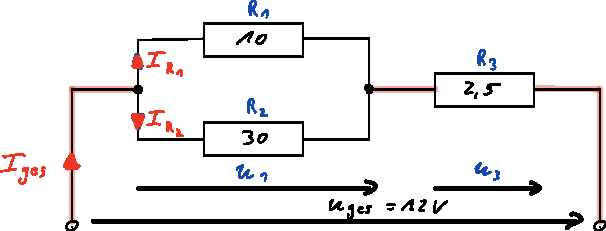
\includegraphics[width=0.6\textwidth]{images/Skizze/25_FM_Nr7_gemischte_Schaltung_A1.pdf}
\caption{FM Nr7 gemischte Schaltung A1}
%\label{fig:}%% anpassen
\end{figure}

\lstset{language=Python}% C, TeX, Bash, Python 
\begin{lstlisting}[
	%caption={}, label={code:}%% anpassen
][language=Python]
# geg: Mathebuch S. 82 Aufgabe 6 Schaltung
R_1 = 10 Ohm
R_2 = 30 Ohm
R_3 = 2,5 Ohm
U_ges = 12 V
# ges: R_I, R_ges, I_ges, U_1, U_3, I_R_1, I_R_2
# Formel:
R_I = 1/(1/R_1 + 1/R_2)
R_ges = R_I + R_3
I_ges = U_ges/R_ges
U_1 = R_I x I_ges
U_3 = R_3 x I_ges
I_R_1 = U_1/R_1
I_R_2 = U_1/R_2
# Lösung:
R_I = 7,5 Ohm
R_ges = 10,0 Ohm
I_ges = 1,2 A
U_1 = 9,0 V
U_3 = 3,0 V
I_R_1 = 0,9 A
I_R_2 = 0,3 A
\end{lstlisting}

\newpage

\textbf{Aufgabe 2}

\begin{figure}[!ht]% hier: !ht
\centering
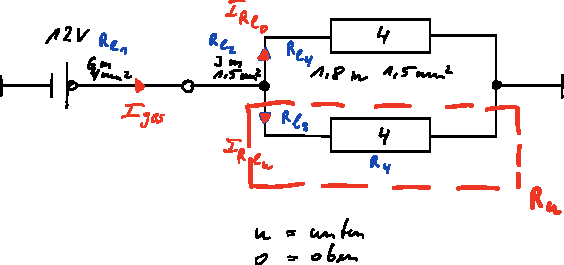
\includegraphics[width=0.6\textwidth]{images/Skizze/25_FM_Nr7_gemischte_Schaltung_A2.pdf}
\caption{FM Nr7 gemischte Schaltung A2}
%\label{fig:}%% anpassen
\end{figure}

\lstset{language=Python}% C, TeX, Bash, Python 
\begin{lstlisting}[
	%caption={}, label={code:}%% anpassen
][language=Python]
# geg: Schaltung
U_ges = 12 V
l_1 = 6 m
A_1 = 4 mm^2
l_2 = 3 m
A_2 = 1,5 mm^2
l_3 = 1,8 m
A_3 = 1,5 mm^2
R_4 = 4 Ohm
p = 0,0178 Kupfer ohm x mm^2 / m 
# ges: U_v_Leitung
# Formel:
R_l_1 = p x l_1 / A_1
R_l_2 = p x l_2 / A_2
R_l_3 = p x l_3 / A_3
R_u = R_l_3 + R_4 (R_o = R_u)
R_II = R_u/2
R_ges = R_l_1 + R_l_2 + R_II
I_ges = U_ges/R_ges
U_v_R_l_3 = R_l_3 x I_R_l_3 -> U_v_R_l_3 = (R_l_3 x I_ges)/2
# Lösung:
R_l_1 = 0,0267 Ohm
R_l_2 = 0,0356 Ohm
R_l_3 = 0,0214 Ohm
R_u = 4,0214 Ohm
R_l_1 = 0,0267 Ohm
R_II = 2,0107 Ohm
R_ges = 2,073 Ohm
I_ges = 5,7888 A
U_v_R_l_3 = 0,0618 V
\end{lstlisting}

\newpage

\textbf{Aufgabe 3}

\begin{figure}[!ht]% hier: !ht
\centering
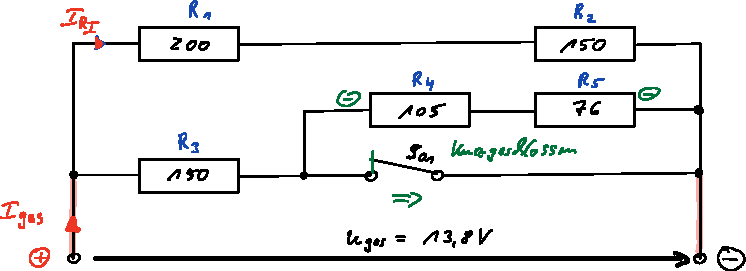
\includegraphics[width=0.6\textwidth]{images/Skizze/25_FM_Nr7_gemischte_Schaltung_A3.pdf}
\caption{FM Nr7 gemischte Schaltung A3}
%\label{fig:}%% anpassen
\end{figure}

\lstset{language=Python}% C, TeX, Bash, Python 
\begin{lstlisting}[
	%caption={}, label={code:}%% anpassen
][language=Python]
# geg: Schaltung
R_1 = 200 Ohm
R_2 = 150 Ohm
R_3 = 150 Ohm
R_4 = 105 Ohm
R_5 = 76 Ohm
U_ges = 13,8 V
# Formel:
# 3,1) ges: R_I, R_II, R_ges_1, R_ges_2, R_delta
R_I = R_1 + R_2
R_II = R_3 + R_4 + R_5 (Schalter offen)
R_ges_1 = 1/(1/R_I + 1/R_II) (Schalter offen)
R_ges_2 = 1/(1/R_II + 1/R_3) (Schalter zu)
R_delta = R_ges_1 - R_ges_2
Gesamtwiderstand ändert sich
# 3,3) ges: I_R_3
I_R_3 = U_ges/R_II (Schalter offen)
# 3,4) ges: U_S_01
U_S_01 = (R_4 + R_5) x I_R_3 (Schalter offen)
# 3,5) ges: I_R_1
I_R_1 = U_ges/R_I
Strom bleibt immer gleich, egal ob Schalter auf/zu
# Lösung:
R_I = 350 Ohm
R_II = 331 Ohm
R_ges_1 = 170,1175 Ohm
R_ges_2 = 103,2225 Ohm
R_delta = 66,895 Ohm
I_R_3 = 0,0417 A
U_S_01 = 7,5462 V
I_R_1 = 0,0394 A
\end{lstlisting}

\newpage

\textbf{Aufgabe 4}

\begin{figure}[!ht]% hier: !ht
\centering
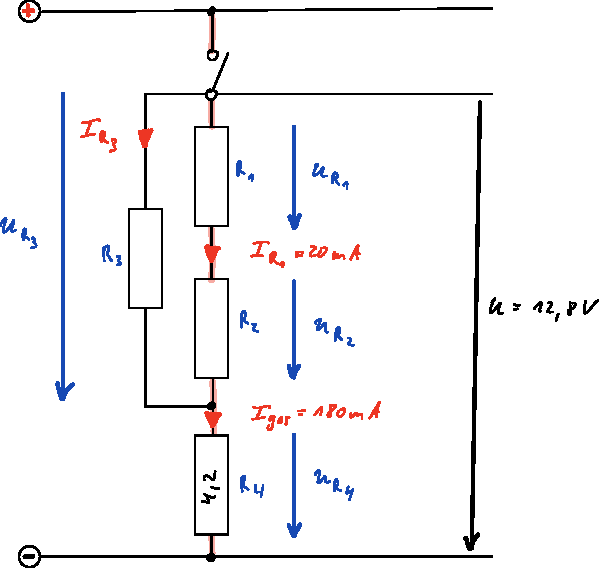
\includegraphics[width=0.6\textwidth]{images/Skizze/25_FM_Nr7_gemischte_Schaltung_A4.pdf}
\caption{FM Nr7 gemischte Schaltung A4}
%\label{fig:}%% anpassen
\end{figure}

\lstset{language=Python}% C, TeX, Bash, Python 
\begin{lstlisting}[
	%caption={}, label={code:}%% anpassen
][language=Python]
# geg: Schaltung
R_4 = 4,2 Ohm
U_ges = 12,8 V
U_R_2 = 1,65 V
I_R_1 = 0,02 A = 20 mA
I_ges = 0,18 A = 180 mA
# ges: R_2, U_R_4, R_1, R_3
# Formel:
R_2 = U_R_2/I_R_1
U_R_4 = R_4 x I_ges
R_1 = U_R_1/I_R_1 -> R_1 = (U_ges - U_R_2 - U_R_4)/I_R_1
R_3 = U_R_3/I_R_3 -> R_3 = (U_ges - U_R_4)/(I_ges - I_R_1)
# Lösung:
R_2 = 82,5 Ohm
U_R_4 = 0,756 V
R_1 = 519,7 Ohm
R_3 = 75,275 Ohm
\end{lstlisting}


	%%%%%%%%%%%%%%%%%%%%%%%%%%%%%%%%%%%%%%%%%%%%%%%%%%%%%%%%%%%%%%%%%%
    % Bibliographie
    \printbibliography
\end{document}
